% GNUPLOT: LaTeX picture with Postscript
\begingroup
  \makeatletter
  \providecommand\color[2][]{%
    \GenericError{(gnuplot) \space\space\space\@spaces}{%
      Package color not loaded in conjunction with
      terminal option `colourtext'%
    }{See the gnuplot documentation for explanation.%
    }{Either use 'blacktext' in gnuplot or load the package
      color.sty in LaTeX.}%
    \renewcommand\color[2][]{}%
  }%
  \providecommand\includegraphics[2][]{%
    \GenericError{(gnuplot) \space\space\space\@spaces}{%
      Package graphicx or graphics not loaded%
    }{See the gnuplot documentation for explanation.%
    }{The gnuplot epslatex terminal needs graphicx.sty or graphics.sty.}%
    \renewcommand\includegraphics[2][]{}%
  }%
  \providecommand\rotatebox[2]{#2}%
  \@ifundefined{ifGPcolor}{%
    \newif\ifGPcolor
    \GPcolortrue
  }{}%
  \@ifundefined{ifGPblacktext}{%
    \newif\ifGPblacktext
    \GPblacktextfalse
  }{}%
  % define a \g@addto@macro without @ in the name:
  \let\gplgaddtomacro\g@addto@macro
  % define empty templates for all commands taking text:
  \gdef\gplbacktext{}%
  \gdef\gplfronttext{}%
  \makeatother
  \ifGPblacktext
    % no textcolor at all
    \def\colorrgb#1{}%
    \def\colorgray#1{}%
  \else
    % gray or color?
    \ifGPcolor
      \def\colorrgb#1{\color[rgb]{#1}}%
      \def\colorgray#1{\color[gray]{#1}}%
      \expandafter\def\csname LTw\endcsname{\color{white}}%
      \expandafter\def\csname LTb\endcsname{\color{black}}%
      \expandafter\def\csname LTa\endcsname{\color{black}}%
      \expandafter\def\csname LT0\endcsname{\color[rgb]{1,0,0}}%
      \expandafter\def\csname LT1\endcsname{\color[rgb]{0,1,0}}%
      \expandafter\def\csname LT2\endcsname{\color[rgb]{0,0,1}}%
      \expandafter\def\csname LT3\endcsname{\color[rgb]{1,0,1}}%
      \expandafter\def\csname LT4\endcsname{\color[rgb]{0,1,1}}%
      \expandafter\def\csname LT5\endcsname{\color[rgb]{1,1,0}}%
      \expandafter\def\csname LT6\endcsname{\color[rgb]{0,0,0}}%
      \expandafter\def\csname LT7\endcsname{\color[rgb]{1,0.3,0}}%
      \expandafter\def\csname LT8\endcsname{\color[rgb]{0.5,0.5,0.5}}%
    \else
      % gray
      \def\colorrgb#1{\color{black}}%
      \def\colorgray#1{\color[gray]{#1}}%
      \expandafter\def\csname LTw\endcsname{\color{white}}%
      \expandafter\def\csname LTb\endcsname{\color{black}}%
      \expandafter\def\csname LTa\endcsname{\color{black}}%
      \expandafter\def\csname LT0\endcsname{\color{black}}%
      \expandafter\def\csname LT1\endcsname{\color{black}}%
      \expandafter\def\csname LT2\endcsname{\color{black}}%
      \expandafter\def\csname LT3\endcsname{\color{black}}%
      \expandafter\def\csname LT4\endcsname{\color{black}}%
      \expandafter\def\csname LT5\endcsname{\color{black}}%
      \expandafter\def\csname LT6\endcsname{\color{black}}%
      \expandafter\def\csname LT7\endcsname{\color{black}}%
      \expandafter\def\csname LT8\endcsname{\color{black}}%
    \fi
  \fi
  \setlength{\unitlength}{0.0500bp}%
  \begin{picture}(9360.00,11520.00)%
      \csname LTb\endcsname%
      \put(4680,11300){\makebox(0,0){\strut{}Verhalten von $R_E$ in Abhängigkeit von $R_1$}}%
    \gplgaddtomacro\gplbacktext{%
      \csname LTb\endcsname%
      \put(1078,7973){\makebox(0,0)[r]{\strut{} 0.52}}%
      \csname LTb\endcsname%
      \put(1078,8417){\makebox(0,0)[r]{\strut{} 0.54}}%
      \csname LTb\endcsname%
      \put(1078,8860){\makebox(0,0)[r]{\strut{} 0.56}}%
      \csname LTb\endcsname%
      \put(1078,9304){\makebox(0,0)[r]{\strut{} 0.58}}%
      \csname LTb\endcsname%
      \put(1078,9748){\makebox(0,0)[r]{\strut{} 0.6}}%
      \csname LTb\endcsname%
      \put(1078,10192){\makebox(0,0)[r]{\strut{} 0.62}}%
      \csname LTb\endcsname%
      \put(1078,10635){\makebox(0,0)[r]{\strut{} 0.64}}%
      \csname LTb\endcsname%
      \put(1078,11079){\makebox(0,0)[r]{\strut{} 0.66}}%
      \csname LTb\endcsname%
      \put(1210,7753){\makebox(0,0){\strut{} 0}}%
      \csname LTb\endcsname%
      \put(1978,7753){\makebox(0,0){\strut{} 5}}%
      \csname LTb\endcsname%
      \put(2747,7753){\makebox(0,0){\strut{} 10}}%
      \csname LTb\endcsname%
      \put(3515,7753){\makebox(0,0){\strut{} 15}}%
      \csname LTb\endcsname%
      \put(4283,7753){\makebox(0,0){\strut{} 20}}%
      \put(176,9526){\rotatebox{-270}{\makebox(0,0){\strut{}Ersatzwiderstand $R_E$ \si{\ohm}}}}%
    }%
    \gplgaddtomacro\gplfronttext{%
    }%
    \gplgaddtomacro\gplbacktext{%
      \csname LTb\endcsname%
      \put(5670,7973){\makebox(0,0)[r]{\strut{} 0.58}}%
      \csname LTb\endcsname%
      \put(5670,8361){\makebox(0,0)[r]{\strut{} 0.581}}%
      \csname LTb\endcsname%
      \put(5670,8750){\makebox(0,0)[r]{\strut{} 0.582}}%
      \csname LTb\endcsname%
      \put(5670,9138){\makebox(0,0)[r]{\strut{} 0.583}}%
      \csname LTb\endcsname%
      \put(5670,9526){\makebox(0,0)[r]{\strut{} 0.584}}%
      \csname LTb\endcsname%
      \put(5670,9914){\makebox(0,0)[r]{\strut{} 0.585}}%
      \csname LTb\endcsname%
      \put(5670,10303){\makebox(0,0)[r]{\strut{} 0.586}}%
      \csname LTb\endcsname%
      \put(5670,10691){\makebox(0,0)[r]{\strut{} 0.587}}%
      \csname LTb\endcsname%
      \put(5670,11079){\makebox(0,0)[r]{\strut{} 0.588}}%
      \csname LTb\endcsname%
      \put(5802,7753){\makebox(0,0){\strut{} 0}}%
      \csname LTb\endcsname%
      \put(6592,7753){\makebox(0,0){\strut{} 5}}%
      \csname LTb\endcsname%
      \put(7383,7753){\makebox(0,0){\strut{} 10}}%
      \csname LTb\endcsname%
      \put(8173,7753){\makebox(0,0){\strut{} 15}}%
      \csname LTb\endcsname%
      \put(8963,7753){\makebox(0,0){\strut{} 20}}%
    }%
    \gplgaddtomacro\gplfronttext{%
    }%
    \gplgaddtomacro\gplbacktext{%
      \csname LTb\endcsname%
      \put(1210,4206){\makebox(0,0)[r]{\strut{} 0.57}}%
      \csname LTb\endcsname%
      \put(1210,4724){\makebox(0,0)[r]{\strut{} 0.575}}%
      \csname LTb\endcsname%
      \put(1210,5242){\makebox(0,0)[r]{\strut{} 0.58}}%
      \csname LTb\endcsname%
      \put(1210,5760){\makebox(0,0)[r]{\strut{} 0.585}}%
      \csname LTb\endcsname%
      \put(1210,6277){\makebox(0,0)[r]{\strut{} 0.59}}%
      \csname LTb\endcsname%
      \put(1210,6795){\makebox(0,0)[r]{\strut{} 0.595}}%
      \csname LTb\endcsname%
      \put(1210,7313){\makebox(0,0)[r]{\strut{} 0.6}}%
      \csname LTb\endcsname%
      \put(1342,3986){\makebox(0,0){\strut{} 0}}%
      \csname LTb\endcsname%
      \put(2077,3986){\makebox(0,0){\strut{} 5}}%
      \csname LTb\endcsname%
      \put(2813,3986){\makebox(0,0){\strut{} 10}}%
      \csname LTb\endcsname%
      \put(3548,3986){\makebox(0,0){\strut{} 15}}%
      \csname LTb\endcsname%
      \put(4283,3986){\makebox(0,0){\strut{} 20}}%
      \put(176,5759){\rotatebox{-270}{\makebox(0,0){\strut{}Ersatzwiderstand $R_E$ \si{\ohm}}}}%
    }%
    \gplgaddtomacro\gplfronttext{%
    }%
    \gplgaddtomacro\gplbacktext{%
      \csname LTb\endcsname%
      \put(5538,4470){\makebox(0,0)[r]{\strut{} 0.5}}%
      \csname LTb\endcsname%
      \put(5538,4786){\makebox(0,0)[r]{\strut{} 0.52}}%
      \csname LTb\endcsname%
      \put(5538,5102){\makebox(0,0)[r]{\strut{} 0.54}}%
      \csname LTb\endcsname%
      \put(5538,5418){\makebox(0,0)[r]{\strut{} 0.56}}%
      \csname LTb\endcsname%
      \put(5538,5734){\makebox(0,0)[r]{\strut{} 0.58}}%
      \csname LTb\endcsname%
      \put(5538,6049){\makebox(0,0)[r]{\strut{} 0.6}}%
      \csname LTb\endcsname%
      \put(5538,6365){\makebox(0,0)[r]{\strut{} 0.62}}%
      \csname LTb\endcsname%
      \put(5538,6681){\makebox(0,0)[r]{\strut{} 0.64}}%
      \csname LTb\endcsname%
      \put(5538,6997){\makebox(0,0)[r]{\strut{} 0.66}}%
      \csname LTb\endcsname%
      \put(5538,7313){\makebox(0,0)[r]{\strut{} 0.68}}%
      \csname LTb\endcsname%
      \put(5670,4250){\makebox(0,0){\strut{} 0}}%
      \csname LTb\endcsname%
      \put(6493,4250){\makebox(0,0){\strut{} 5}}%
      \csname LTb\endcsname%
      \put(7317,4250){\makebox(0,0){\strut{} 10}}%
      \csname LTb\endcsname%
      \put(8140,4250){\makebox(0,0){\strut{} 15}}%
      \csname LTb\endcsname%
      \put(8963,4250){\makebox(0,0){\strut{} 20}}%
      \put(7316,3920){\makebox(0,0){\strut{}Widerstandswert von $R_1$ /\si{\ohm}}}%
    }%
    \gplgaddtomacro\gplfronttext{%
    }%
    \gplgaddtomacro\gplbacktext{%
      \csname LTb\endcsname%
      \put(946,704){\makebox(0,0)[r]{\strut{} 0}}%
      \csname LTb\endcsname%
      \put(946,1110){\makebox(0,0)[r]{\strut{} 0.2}}%
      \csname LTb\endcsname%
      \put(946,1516){\makebox(0,0)[r]{\strut{} 0.4}}%
      \csname LTb\endcsname%
      \put(946,1922){\makebox(0,0)[r]{\strut{} 0.6}}%
      \csname LTb\endcsname%
      \put(946,2328){\makebox(0,0)[r]{\strut{} 0.8}}%
      \csname LTb\endcsname%
      \put(946,2734){\makebox(0,0)[r]{\strut{} 1}}%
      \csname LTb\endcsname%
      \put(946,3140){\makebox(0,0)[r]{\strut{} 1.2}}%
      \csname LTb\endcsname%
      \put(946,3546){\makebox(0,0)[r]{\strut{} 1.4}}%
      \csname LTb\endcsname%
      \put(1078,484){\makebox(0,0){\strut{} 0}}%
      \csname LTb\endcsname%
      \put(1879,484){\makebox(0,0){\strut{} 5}}%
      \csname LTb\endcsname%
      \put(2681,484){\makebox(0,0){\strut{} 10}}%
      \csname LTb\endcsname%
      \put(3482,484){\makebox(0,0){\strut{} 15}}%
      \csname LTb\endcsname%
      \put(4283,484){\makebox(0,0){\strut{} 20}}%
      \put(176,2125){\rotatebox{-270}{\makebox(0,0){\strut{}Ersatzwiderstand $R_E$ \si{\ohm}}}}%
      \put(2680,154){\makebox(0,0){\strut{}Widerstandswert von $R_1$ /\si{\ohm}}}%
    }%
    \gplgaddtomacro\gplfronttext{%
    }%
    \gplbacktext
    \put(0,0){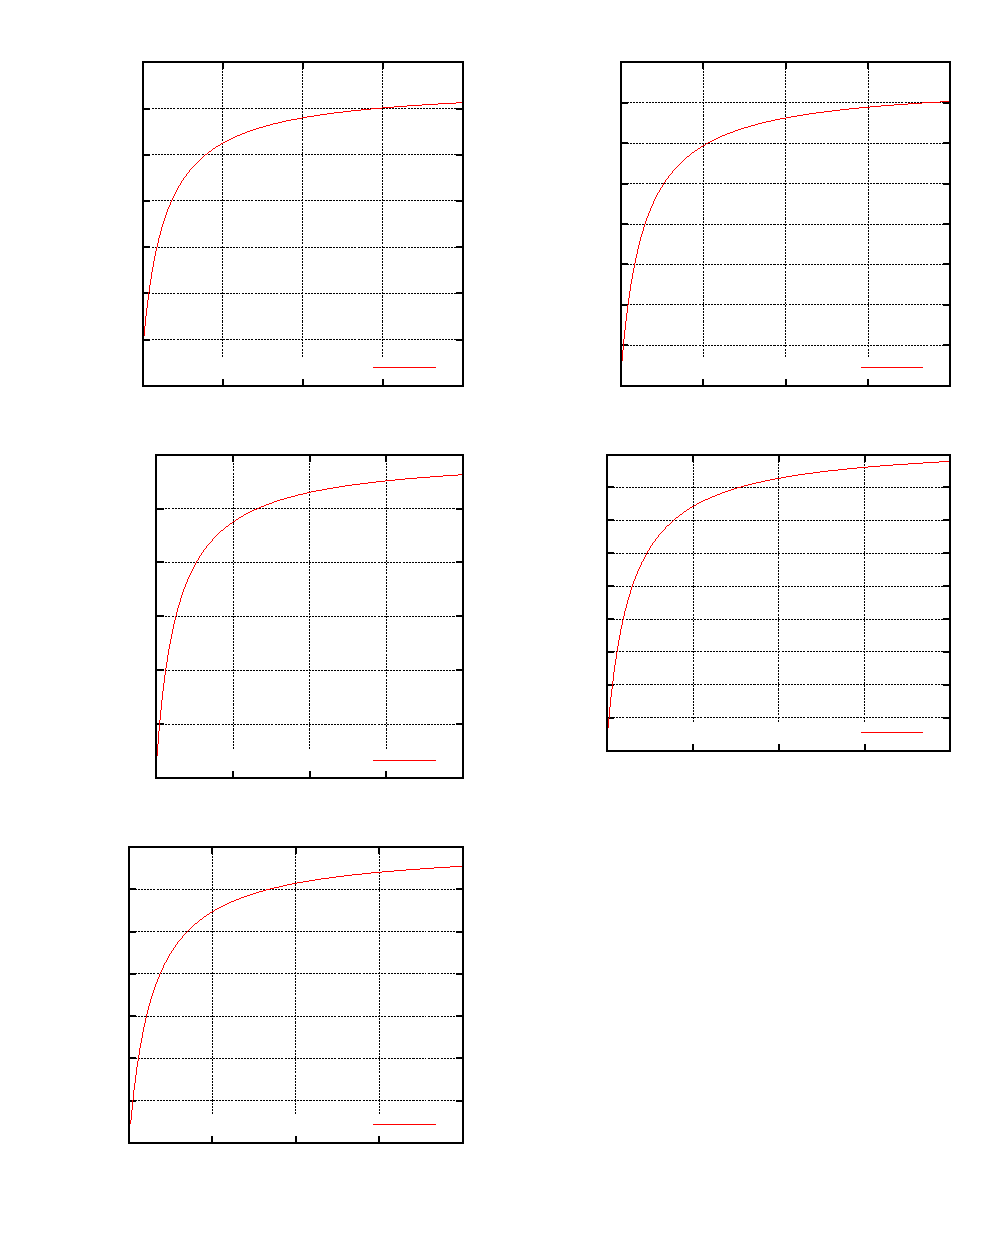
\includegraphics{./figures/wuerfel_edge}}%
    \gplfronttext
  \end{picture}%
\endgroup
